\documentclass[tikz,border=8pt]{standalone}
% Shared look for every TikZ diagram. Load with % Shared look for every TikZ diagram. Load with % Shared look for every TikZ diagram. Load with \input{../../tools/tikz-style.tex}
\usepackage[T1]{fontenc}
\usepackage{lmodern}
\renewcommand{\sfdefault}{lmr}  % diagrams use the same serif as the text
\usetikzlibrary{arrows.meta, positioning, shapes.geometric, calc, fit, backgrounds}
\definecolor{cblue}{HTML}{4C78A8}
\definecolor{corange}{HTML}{F58518}
\definecolor{cgreen}{HTML}{54A24B}
\definecolor{cred}{HTML}{E45756}
\definecolor{cpurple}{HTML}{B279A2}
\definecolor{cgrey}{HTML}{6B6B6B}
\tikzset{
  every picture/.style={font=\sffamily, line width=1.2pt},
  box/.style={draw=#1, fill=#1!12, rounded corners=4pt, align=center, inner sep=7pt, minimum height=1.1cm},
  box/.default=cgrey,
  arrow/.style={-{Stealth[length=3mm]}, draw=cgrey, line width=1.4pt},
  title/.style={font=\sffamily\bfseries\Large},
  note/.style={font=\sffamily\small, text=cgrey, align=center},
}
\AtBeginDocument{\hyphenpenalty=10000 \exhyphenpenalty=10000}

\usepackage[T1]{fontenc}
\usepackage{lmodern}
\renewcommand{\sfdefault}{lmr}  % diagrams use the same serif as the text
\usetikzlibrary{arrows.meta, positioning, shapes.geometric, calc, fit, backgrounds}
\definecolor{cblue}{HTML}{4C78A8}
\definecolor{corange}{HTML}{F58518}
\definecolor{cgreen}{HTML}{54A24B}
\definecolor{cred}{HTML}{E45756}
\definecolor{cpurple}{HTML}{B279A2}
\definecolor{cgrey}{HTML}{6B6B6B}
\tikzset{
  every picture/.style={font=\sffamily, line width=1.2pt},
  box/.style={draw=#1, fill=#1!12, rounded corners=4pt, align=center, inner sep=7pt, minimum height=1.1cm},
  box/.default=cgrey,
  arrow/.style={-{Stealth[length=3mm]}, draw=cgrey, line width=1.4pt},
  title/.style={font=\sffamily\bfseries\Large},
  note/.style={font=\sffamily\small, text=cgrey, align=center},
}
\AtBeginDocument{\hyphenpenalty=10000 \exhyphenpenalty=10000}

\usepackage[T1]{fontenc}
\usepackage{lmodern}
\renewcommand{\sfdefault}{lmr}  % diagrams use the same serif as the text
\usetikzlibrary{arrows.meta, positioning, shapes.geometric, calc, fit, backgrounds}
\definecolor{cblue}{HTML}{4C78A8}
\definecolor{corange}{HTML}{F58518}
\definecolor{cgreen}{HTML}{54A24B}
\definecolor{cred}{HTML}{E45756}
\definecolor{cpurple}{HTML}{B279A2}
\definecolor{cgrey}{HTML}{6B6B6B}
\tikzset{
  every picture/.style={font=\sffamily, line width=1.2pt},
  box/.style={draw=#1, fill=#1!12, rounded corners=4pt, align=center, inner sep=7pt, minimum height=1.1cm},
  box/.default=cgrey,
  arrow/.style={-{Stealth[length=3mm]}, draw=cgrey, line width=1.4pt},
  title/.style={font=\sffamily\bfseries\Large},
  note/.style={font=\sffamily\small, text=cgrey, align=center},
}
\AtBeginDocument{\hyphenpenalty=10000 \exhyphenpenalty=10000}

\begin{document}
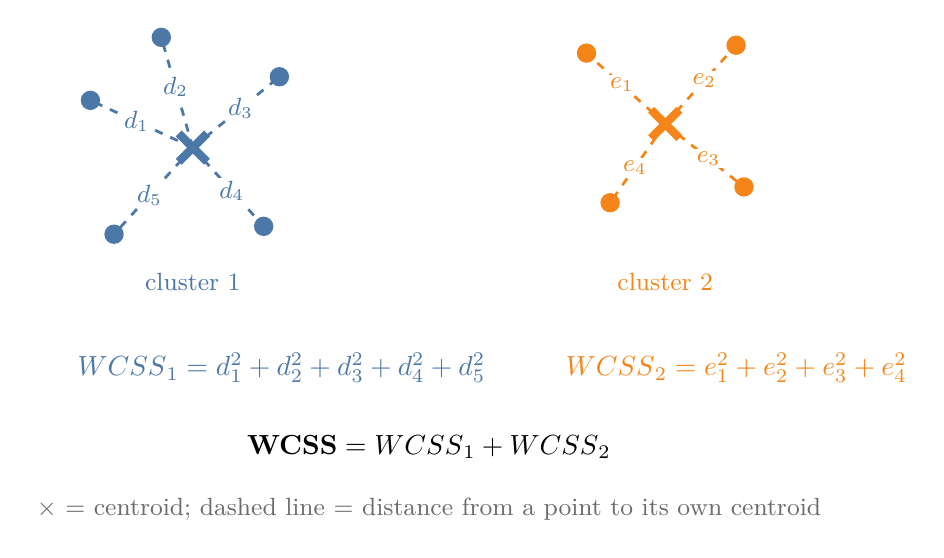
\begin{tikzpicture}
  % cluster 1
  \coordinate (c1) at (0,0);
  \foreach \p/\n in {(-1.3,0.6)/1,(-0.4,1.4)/2,(1.1,0.9)/3,(0.9,-1.0)/4,(-1.0,-1.1)/5} {
    \draw[cblue, dashed, line width=1pt] (c1) -- \p node[pos=0.55, fill=white, inner sep=1pt, font=\small, text=cblue] {$d_\n$};
    \fill[cblue] \p circle (3.5pt);
  }
  \draw[cblue, line width=3pt] ($(c1)+(-0.18,-0.18)$) -- ($(c1)+(0.18,0.18)$) ($(c1)+(-0.18,0.18)$) -- ($(c1)+(0.18,-0.18)$);
  \node[font=\small, text=cblue] at (0,-1.7) {cluster 1};
  % cluster 2
  \coordinate (c2) at (6,0.3);
  \foreach \p/\n in {(5.0,1.2)/1,(6.9,1.3)/2,(7.0,-0.5)/3,(5.3,-0.7)/4} {
    \draw[corange, dashed, line width=1pt] (c2) -- \p node[pos=0.55, fill=white, inner sep=1pt, font=\small, text=corange] {$e_\n$};
    \fill[corange] \p circle (3.5pt);
  }
  \draw[corange, line width=3pt] ($(c2)+(-0.18,-0.18)$) -- ($(c2)+(0.18,0.18)$) ($(c2)+(-0.18,0.18)$) -- ($(c2)+(0.18,-0.18)$);
  \node[font=\small, text=corange] at (6,-1.7) {cluster 2};
  % formulas
  \node[text=cblue, anchor=west] at (-1.6,-2.8) {$\text{WCSS}_1 = d_1^2 + d_2^2 + d_3^2 + d_4^2 + d_5^2$};
  \node[text=corange, anchor=west] at (4.6,-2.8) {$\text{WCSS}_2 = e_1^2 + e_2^2 + e_3^2 + e_4^2$};
  \node[anchor=center] at (3,-3.8) {$\textbf{WCSS} = \text{WCSS}_1 + \text{WCSS}_2$};
  \node[note] at (3,-4.6) {$\times$ = centroid; dashed line = distance from a point to its own centroid};
\end{tikzpicture}
\end{document}
